This project investigates whether biologically inspired spiking neural network can be used to recognise and track shapes in a video stream in real time. 

In this chapter a brief introduction on the functioning of biological neurons and the technologies used in order to simulate them will be presented. A quick discussion on the motivation and previous work in the area will also provided. 

\section{Neuron}
Neurons are highly specialised cells found in the nervous system designed to generate and transmit electrical signals to other cells. Many different kinds of neurons exist \cite{Llinas:2008}, each with different morphology, but a typical neuron can be divided in three parts shown in \cref{fig:neuron_morphology} \textbf{A}:
\begin{itemize}
    \item Soma: a usually compact area which represents the body of the neuron and which contains the cell nucleus.
    \item Dendrites: tree-like extensions of the soma membrane which acts as the ``input'' pole to the neuron.
    \item Axons: a cable-like structure that acts as the ``output'' pole of the neuron and propagate neuronal output to other cells.
\end{itemize}
The axon of a \textit{presynaptic cell} makes contact with the dendrite of a \textit{postsynaptic cell} at a site called synapse \cite{Gerstner:2014}, highlighted in \cref{fig:neuron_morphology} \textbf{B}.

\begin{figure}[ht]
\centering
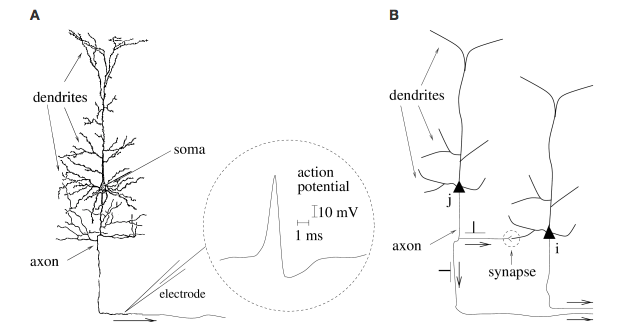
\includegraphics[scale=0.6]{images/neuron.png}
\caption[Neuron Morphology]{\textbf{A}. A cortical pyramidal cell with its soma, axon and dendrites highlighted. \textbf{B}. Signal transmission from neuron $j$ (presynaptic cell) to neuron $i$ (postsynaptic cell). Reproduced from \cite{Gerstner:2014}.}
\label{fig:neuron_morphology}
\end{figure}

A neuron spikes when the current input carried by the dendrites exceeds a certain threshold. The biochemical details of this process are not relevant for this project and the variety in electrophysiological properties of neurons \cite{Llinas:2008} leads to necessary simplification in order to simulate them. The signals emitted by neurons are called action potentials or spikes, and an approximate form is shown in the circled area of  \cref{fig:neuron_morphology}. A key property of action potential is that the form does not carry any information, information is actually carried by the number of action potentials and their timings \cite{Gerstner:2014}. After each spike the neuron enters a state called refractory period, in which it is impossible for it to spike again.  

Several mathematical models are available in order to simulate neurons, the one used in this project is a leaky integrate-and-fire (LIF) neuron model. 

% TODO insert maths details of LIF model


\section{SpiNNaker}
In order to handle the obvious complexity of neural simulation two approaches are possible. The first one is to use supercomputer built for general purpose task like in the case of the Blue Brain project which uses IBM's Blue Gene supercomputers \cite{Markram2006}. The second approach is to employ neuromorphic systems. These systems are designed around the idea that small computing elements (the ``neurons'') perform computation in a highly distributed manner in ways that mimic biological brains \cite{Furber2016}. Several of these systems have been developed recently, for example IBM TrueNorth, Stanford Neurogrid and University of Manchester SpiNNaker, which will be the system used for this project.

SpiNNaker is a massively-parallel multi-core computing system designed for large scale brain simulations running in biological real time. The system had been designed focusing on scalability, in order to model the very large number of components in a biological brain, and energy efficiency.

\begin{figure}[ht]
\centering
\begin{subfigure}{0.45\textwidth}
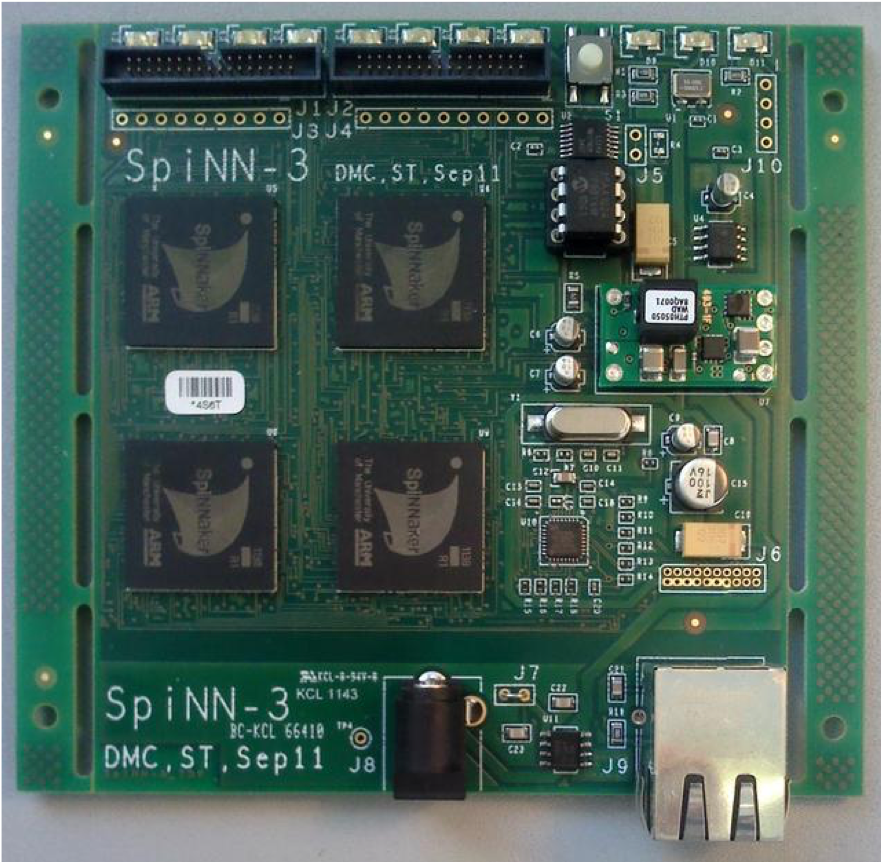
\includegraphics[width=\textwidth]{images/spinnaker_board.png} 
\caption{SpiNNaker board with 4 chips.}
\label{fig:spinnaker_board}
\imagesource{http://apt.cs.manchester.ac.uk/projects/SpiNNaker/hardware/index3.php}
\end{subfigure}
\begin{subfigure}{0.45\textwidth}
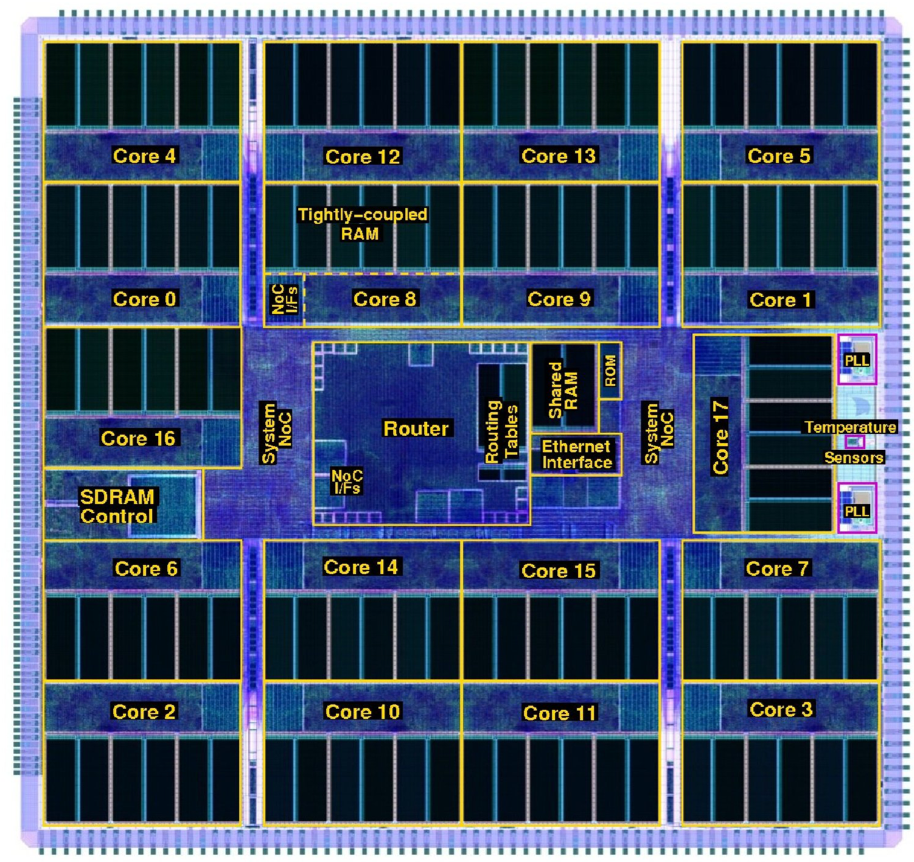
\includegraphics[width=\textwidth]{images/spinnaker_chip.png}
\caption{SpiNNaker chip}
\label{fig:spinnaker_chip}
\imagesource{http://apt.cs.manchester.ac.uk/projects/SpiNNaker/SpiNNchip}
\end{subfigure}
\caption[SpiNNaker Board and Chip]{SpiNNaker board and chip}
\label{fig:spinnaker}
\end{figure}

SpiNNaker is available at different scale, from a 4 chips board shown in \cref{fig:spinnaker_board} to a 1,036,800 cores machine accessible through the Neuromorphic Computing platform of the Human Brain Project \footnote{\url{https://www.humanbrainproject.eu/en/silicon-brains/} --- Accessed 19 April 2019}.

For this project, a 4 chips board has been used. Each chip, \cref{fig:spinnaker_chip} includes 18 ARM9 cores and \SI{128}{\mega\byte} of SDRAM. The board is connected to a host machine through an Ethernet cable and it is powered through a \SI{5}{\volt} \SI{1}{\ampere} USB cable.

\section{Dynamic Vision Sensor}


\section{Motivation}


\section{Previous Work}
